% DRAFT started in Week 9. Results and Discussion are drafted. The other sections
% are shortened from the mid-sem report and need a final pass in Week 10.
\documentclass[conference]{IEEEtran}
\usepackage{graphicx}
\usepackage{booktabs}
\usepackage{amsmath}
\usepackage{cite}
\graphicspath{{../Results/final/}{../Results/analysis/}{../Results/real_fields/}}

\begin{document}

\title{SAR and Optical Feature Fusion for Crop Classification Using YieldSAT}

\author{\IEEEauthorblockN{Het Patel (AU2440266), Dhairya Shah (AU2440128), Jay Daftari (AU2440271), Hiya Soni (AU2440084)}
\IEEEauthorblockA{ECE 501 Digital Image Processing, Project 19, Group 3\\
Ahmedabad University\\
Code: github.com/Het1236/DIP\_2026\_19\_3}}

\maketitle

\begin{abstract}
% TODO Week 10: final pass after the numbers are locked.
We study crop classification from optical and radar satellite images together. We use the YieldSAT dataset for Argentina and Brazil. We build a pipeline that removes clouds from Sentinel-2 images and reduces speckle in Sentinel-1 images. From 270 real fields we extract vegetation indices, radar backscatter statistics and texture features. We train Random Forest and SVM models on optical-only, SAR-only and fused features. Fused features give the best result. In nested 5-fold cross validation the fused SVM reaches a macro F1-score of 0.91 and the best single image type reaches 0.81. On one held-out test split the fused Random Forest reaches 0.93. A model trained on one country does not work well on the other, and its macro F1-score falls to about 0.48.
\end{abstract}

\begin{IEEEkeywords}
crop classification, SAR, optical, feature fusion, Sentinel-1, Sentinel-2, YieldSAT
\end{IEEEkeywords}

\section{Introduction}
% TODO Week 10: shorten the mid-sem introduction and state the research question.
Knowing which crop grows in a field helps with farm planning and food security. Optical satellites are easy to read but clouds block the view. Radar satellites work through clouds but their images are noisy. In our real fields the cloud mask kept only about 55\% of the optical dates. We ask whether features from both image types together classify crops better than features from either one alone.

We use classical hand-crafted features and classical machine learning. We do not use deep learning. We use the YieldSAT dataset \cite{yieldsat}. Our group was assigned Argentina and Brazil.

\section{Methodology}
% TODO Week 10: add one pipeline figure and check the equations against the mid-sem report.
\subsection{Data and preprocessing}
YieldSAT has 751 fields for Argentina and 551 for Brazil. It has Sentinel-2 images and crop labels but no radar data. We download Sentinel-1 data for the same fields through Google Earth Engine \cite{gee}. For the optical images we keep clear pixels using the scene classification layer. We build a median composite from the middle part of the season, from 30\% to 70\% of the way between seeding and harvest. For the radar images we take the median of the scenes, apply a $5\times5$ Lee filter \cite{lee} and align the result to the optical grid.

\subsection{Features}
From each field we compute the means of four vegetation indices: NDVI \cite{rouse}, EVI, GNDVI and NDWI. From the radar images we compute the mean and standard deviation of VV and VH and the VV minus VH difference. We also compute four texture features from the gray level co-occurrence matrix \cite{haralick}: contrast, homogeneity, energy and correlation. They are computed on NIR, NDVI, VV and VH. This gives 12 optical features and 13 SAR features.

\subsection{Fusion and models}
Fusion is early fusion. We join the optical and SAR features into one vector. We then drop one feature from each pair with a correlation above 0.95. This step uses the training data only. It reduces the 25 features to 21. We train a Random Forest and an SVM with an RBF kernel. Hyperparameters are chosen by 5-fold cross validation on the training data, scored by macro F1-score. The same search is used for all three feature sets.

\section{Results}
\subsection{Experimental setup}
We sampled 50 fields for each country and crop, using fields with Good or Average quality. This gives 300 fields. Features were built for 270 of them. Of the other 30, 16 had no Sentinel-1 scenes in their date range, 11 were too cloudy, 2 had no Sentinel-2 date inside the season window and 1 failed because of a server error. The 270 fields are 133 from Argentina and 137 from Brazil. They contain 91 corn, 88 soybean and 91 wheat fields. We split them 80\% and 20\% with the same crop mix in both parts. This gives 216 training and 54 test fields. Each crop has 18 test fields.

\subsection{Optical-only, SAR-only and fused features}
Table~\ref{tab:main} and Fig.~\ref{fig:bars} show the test results. Fused features give the best result for both models. The fused Random Forest has an accuracy of 0.93 and gets 50 of the 54 test fields right. The best single-type model is the SAR Random Forest, with an accuracy of 0.80 and 43 of 54 correct. Optical features give the lowest result with Random Forest.

\begin{table}[t]
\caption{Test-set results (54 fields) after tuning.}
\label{tab:main}
\centering
\footnotesize
\setlength{\tabcolsep}{4pt}
\begin{tabular}{llccc}
\toprule
Features & Model & \# feat. & Acc. & Macro F1\\
\midrule
Optical & RF  & 12 & 0.65 & 0.63\\
Optical & SVM & 12 & 0.76 & 0.76\\
SAR     & RF  & 13 & 0.80 & 0.79\\
SAR     & SVM & 13 & 0.76 & 0.76\\
Fused   & RF  & 21 & \textbf{0.93} & \textbf{0.93}\\
Fused   & SVM & 21 & 0.91 & 0.91\\
\bottomrule
\end{tabular}
\end{table}

\begin{figure}[t]
\centering
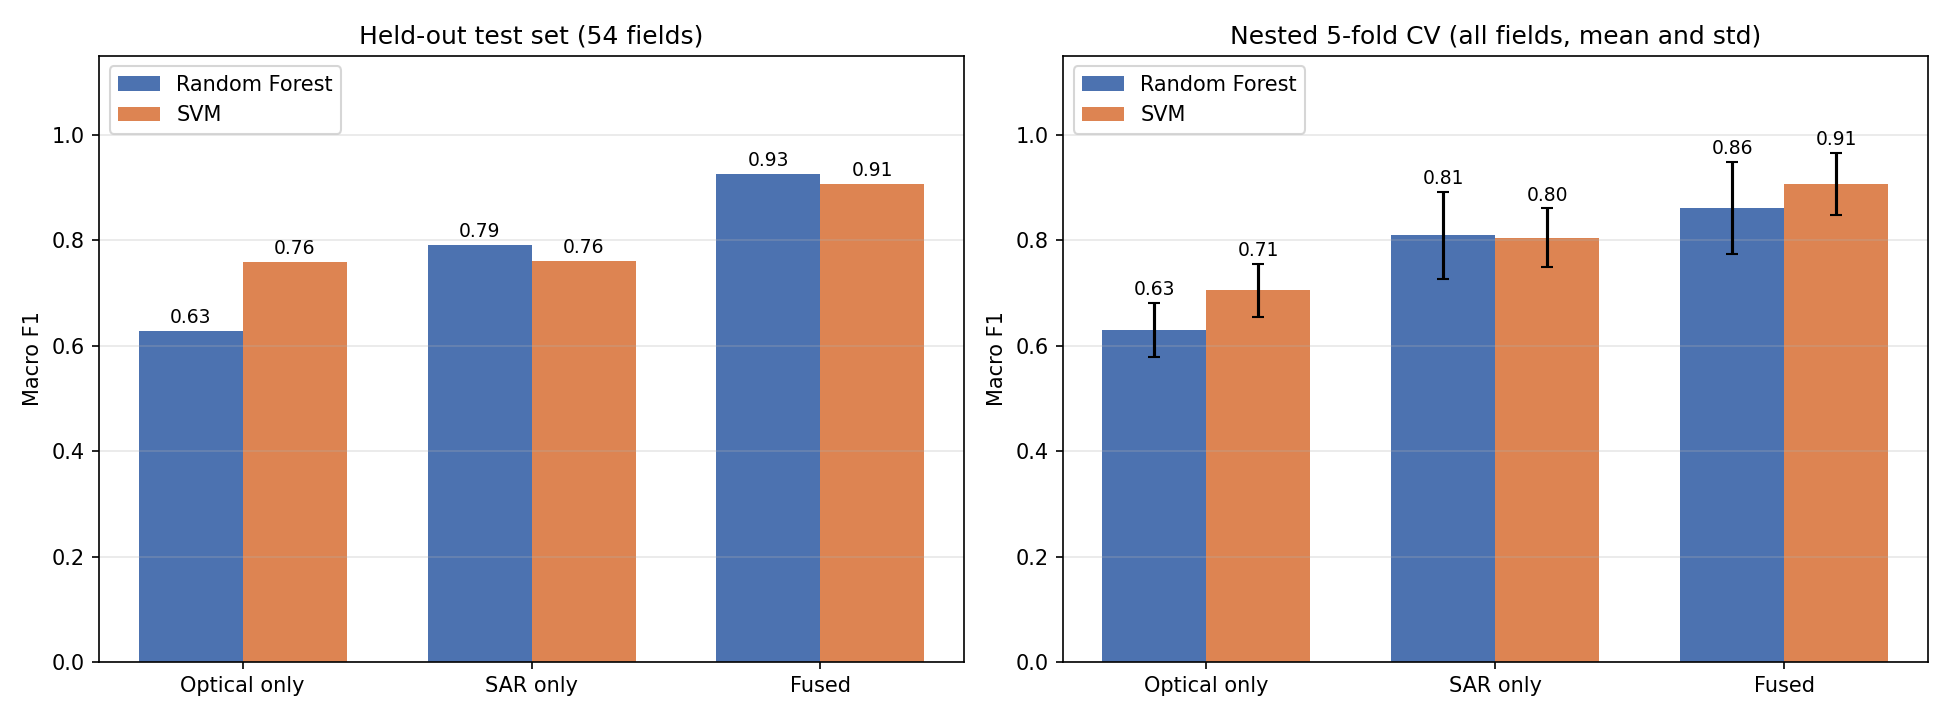
\includegraphics[width=\columnwidth]{final_comparison_bars.png}
\caption{Macro F1-score by feature set and model. Left: held-out test set. Right: nested 5-fold cross validation over all 270 fields.}
\label{fig:bars}
\end{figure}

\subsection{Nested cross validation}
With 54 test fields, one field changes the accuracy by about 2\%. To check that the result does not depend on one split, we ran a nested 5-fold cross validation over all 270 fields. The tuning and the correlation filter use only the training part of each fold. Table~\ref{tab:cv} gives the mean and the standard deviation over the 5 folds. The fused SVM has the best result, a macro F1-score of 0.91. The best single-type models are the SAR ones, with 0.81 for Random Forest and 0.80 for SVM. Optical features reach 0.63 with Random Forest and 0.71 with SVM. The fused SVM is about 0.10 above the best single-type model. The fused Random Forest is only about 0.05 above it, and this is smaller than the spread between folds (0.08 to 0.09).

\begin{table}[t]
\caption{Nested 5-fold cross validation over all 270 fields (mean $\pm$ std).}
\label{tab:cv}
\centering
\footnotesize
\begin{tabular}{llcc}
\toprule
Features & Model & Accuracy & Macro F1\\
\midrule
Optical & RF & 0.63 $\pm$ 0.05 & 0.63 $\pm$ 0.05\\
Optical & SVM & 0.70 $\pm$ 0.05 & 0.71 $\pm$ 0.05\\
SAR & RF & 0.81 $\pm$ 0.08 & 0.81 $\pm$ 0.08\\
SAR & SVM & 0.81 $\pm$ 0.06 & 0.80 $\pm$ 0.06\\
Fused & RF & 0.86 $\pm$ 0.09 & 0.86 $\pm$ 0.09\\
Fused & SVM & \textbf{0.91} $\pm$ 0.06 & \textbf{0.91} $\pm$ 0.06\\
\bottomrule
\end{tabular}
\end{table}

\subsection{Error analysis}
Fig.~\ref{fig:cm} shows the confusion matrices. For the fused Random Forest the macro F1-scores are 0.91 for corn, 0.92 for soybean and 0.94 for wheat. No crop is clearly weak. The accuracy is 0.88 for Argentina (21 of 24 fields) and 0.97 for Brazil (29 of 30 fields). This gap is 2 fields, so we do not treat it as a real difference.

\begin{figure*}[t]
\centering
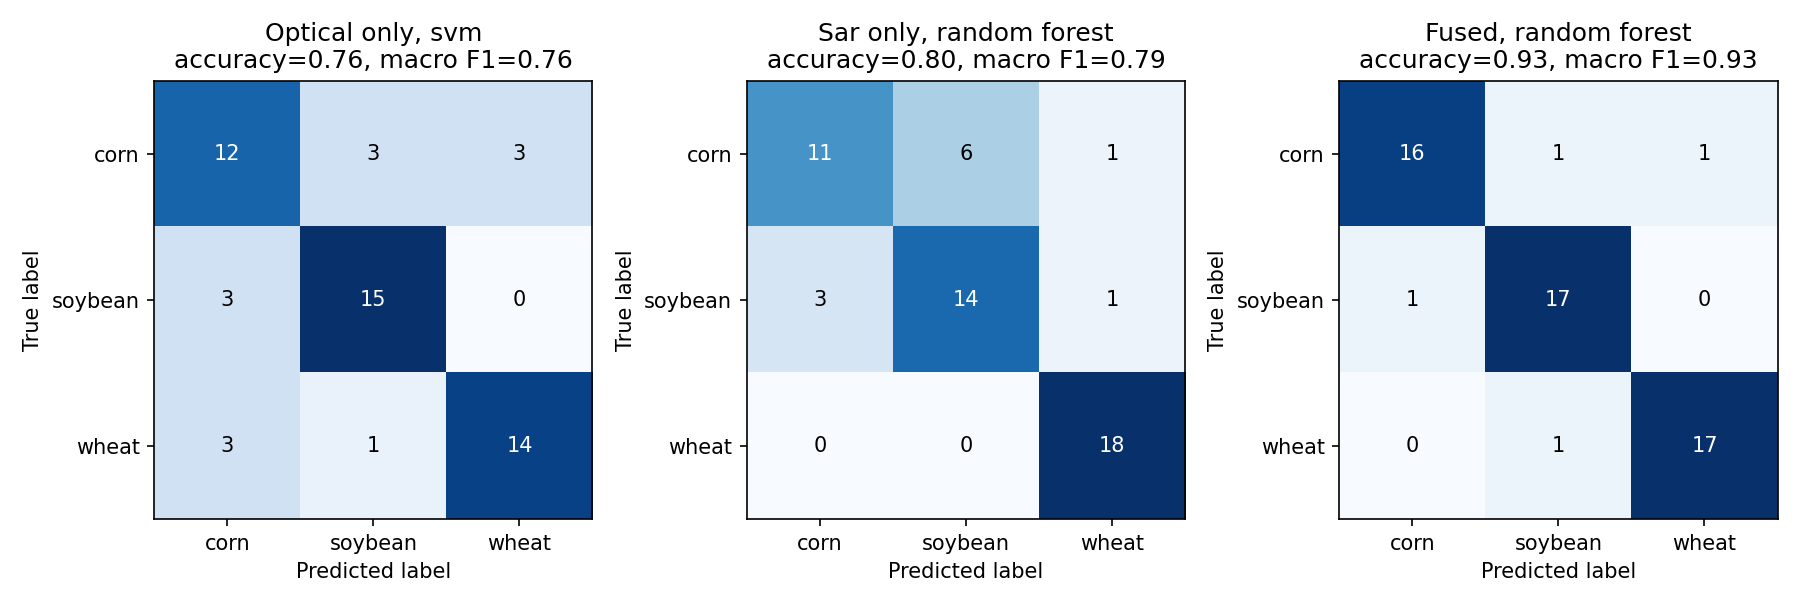
\includegraphics[width=0.85\textwidth]{final_confusion_matrices.png}
\caption{Confusion matrices on the test set for the best model of each feature set.}
\label{fig:cm}
\end{figure*}

The most important features are the mean VV and the VV minus VH difference, both from SAR. The mean EVI is third. SAR features hold 65\% of the total importance and optical features hold 35\%. Simple mean values matter more than texture features. The best texture feature is the NIR correlation with an importance of about 0.06.

\subsection{Cross-country test}
We trained on one country and tested on the other (Table~\ref{tab:cross}). The accuracy is 0.52 for Argentina to Brazil and 0.45 for Brazil to Argentina. The macro F1-score falls from 0.93 on the mixed test set to about 0.48. Random guessing among three crops gives about 0.33.

\begin{table}[t]
\caption{Train on one country, test on the other (fused Random Forest).}
\label{tab:cross}
\centering
\footnotesize
\begin{tabular}{llccc}
\toprule
Train & Test & \# train & Acc. & Macro F1\\
\midrule
Argentina & Brazil    & 133 & 0.52 & 0.51\\
Brazil    & Argentina & 137 & 0.45 & 0.44\\
\bottomrule
\end{tabular}
\end{table}

\section{Discussion}
Fusion helped. In nested cross validation the best fused model has a macro F1-score of 0.91 and the best single-type model has 0.81. The fused model uses both types, since its top features come from SAR and from optical.

The size of the gain needs care. On the single test split the gain was larger, 0.93 against 0.79, so that split is probably on the high side. The gain is about 0.10 for the SVM and about 0.05 for the Random Forest, and the Random Forest value is inside the spread between folds. The test split and the cross validation also disagree on the best fused model. We therefore report the gain as a real but modest improvement and do not name one best model.

SAR features did better than optical features in our data. A possible reason is that radar is not blocked by clouds, so the SAR features are built from complete data. We have not tested this explanation.

The cross-country result is the main limit of our work. The model works well inside the mixed data but does not carry over to a new country. The YieldSAT authors also report that models lose accuracy on new regions \cite{yieldsat}. A likely reason is that the two countries have different seasons, climate and farming, so the same crop gives different feature values. We have not tested this. Our cross-country models also train on only 133 or 137 fields.

Other limits are the small test set, a single split in the main table, and the use of 270 of the 1302 fields.

\section{Conclusion}
% TODO Week 10: final wording once all numbers are locked.
We built a pipeline that turns Sentinel-2 and Sentinel-1 images into field features and tested optical-only, SAR-only and fused classification of corn, soybean and wheat. Fused features gave the best macro F1-score. In nested cross validation it was 0.91 for the fused SVM against 0.81 for the best single image type. The models did not carry over from one country to the other. Future work is to use more fields, to test why the countries differ and to try adapting the features to a new country.

\begin{thebibliography}{9}
\bibitem{yieldsat} M. Miranda \textit{et al.}, ``YieldSAT: A multimodal benchmark dataset for high-resolution crop yield prediction,'' in \textit{Proc. IEEE/CVF Conf. Computer Vision and Pattern Recognition (CVPR)}, 2026, arXiv:2604.00940.
\bibitem{gee} N. Gorelick \textit{et al.}, ``Google Earth Engine: Planetary-scale geospatial analysis for everyone,'' \textit{Remote Sens. Environ.}, vol. 202, pp. 18--27, 2017.
\bibitem{lee} J.-S. Lee, ``Digital image enhancement and noise filtering by use of local statistics,'' \textit{IEEE Trans. Pattern Anal. Mach. Intell.}, vol. PAMI-2, no. 2, pp. 165--168, Mar. 1980.
\bibitem{rouse} J. W. Rouse \textit{et al.}, ``Monitoring vegetation systems in the Great Plains with ERTS,'' in \textit{Proc. 3rd ERTS Symp.}, NASA SP-351, 1974, pp. 309--317.
\bibitem{haralick} R. M. Haralick, K. Shanmugam, and I. Dinstein, ``Textural features for image classification,'' \textit{IEEE Trans. Syst., Man, Cybern.}, vol. SMC-3, no. 6, pp. 610--621, Nov. 1973.
\end{thebibliography}

\end{document}
